\section{The bow of the readout boards: details}\label{app:bow}
\sectionstate{partial}{the old section 7.5 less what is now in \cref{sec:bow}; \texttt{rerun/model\_audit/followups/fb\_bow\_maps/}
(numbers re-run on the final tables 2026-11-03); corrections from the bow agent's report (2--29\,\%, the fringe sentence).}
\intent{This appendix answers one question: is the bow real, or could something else produce the three signals? It
gives the estimator, the sign, the alternatives excluded, the stability across runs, a plausibility estimate and the
correction with its transfer to the beam.}

\subsection{The three observables in detail}
(i)~\emph{Positions.} A track of slope $\tan\theta = \mathrm{d}x/\mathrm{d}z$ crosses a mesh displaced by $h$ along $z$
at a point shifted by $h\tan\theta$. In every position cell the slope of the position residual (fitted mesh position
minus the reference prediction) against the reference slope is therefore the local mesh height $h(x,y)$. It is measured independently
by the X and the Y strips, through the two independent reference projections. All numbers of this appendix and of \cref{sec:bow} come from one
estimator, run on the long runs: an event-level robust fit of
the position residual to $\tan\theta\,h(u,w)$ with $h$ a quadratic surface of the track position at mid-gap, and of the fitted
transverse rate to a quadratic surface plus a term proportional to the reference slope, for each view; the dish depth
pools its four curvature terms. Both views see a dish in both directions
(\cref{fig:bowprof}): the centre lies $1.3$--$1.9$\,mm below a point 150\,mm out
(B $1.87\pm0.24$, A $1.31\pm0.22$, E $1.69\pm0.22$, C $1.76\pm0.18$, D $1.68\pm0.23$\,mm), i.e.\ a mean curvature of
$1.2$--$1.7\times10^{-4}$\,mm$^{-1}$. Each error combines, in quadrature, the bootstrap error of the pooled depth ($0.06$--$0.11$\,mm)
and the standard error of the mean of the four terms (their scatter divided by $\sqrt4$, $0.17$--$0.22$\,mm). The four terms of one chamber, two
per view, scatter by $0.3$--$0.4$\,mm at 150\,mm, which is the uncertainty of a single term. They share the telescope and the board, so the
combined error is a floor, and a bow common to the reference planes is not in it (below).
The X strips read $1.2$--$1.8$\,mm and the Y strips $1.5$--$1.9$\,mm; neither view is deeper on every chamber
(Y deeper on A, B, C; X deeper on D, E). Along $y$ the dish is $0.15$--$0.7$\,mm deeper than along $x$ on all five chambers
(at 150\,mm, $1.7$--$2.1$ against $1.0$--$1.8$\,mm; a mean ratio of curvatures of 1.4, range 1.0--1.6). This is a measured tendency, not a claim of
anisotropy of the board: the drift-tilt ramp below, which does not depend on the telescope's depth, points the same way, but with five chambers
the two are only weakly correlated ($r=0.57$) and a bow of the reference planes along $y$ could contribute to the position route. \Cref{fig:bowprof} draws the
fitted quadratic surface itself, along both axes through the centre, for each view and each chamber, with the pooled dish and its combined error;
the data behind it are in \crefp{fig:bow}{a, b} for chamber~A. The dish is not a pure parabola: the drift-tilt gradient depends on the part of the chamber fitted (below), so the quadratic is a description of the
central region.
(ii)~\emph{Drift tilt.} If drift lines leave the mesh normal to its surface, charge produced at height $d$ arrives
displaced by $d\,\partial h/\partial x$, so the fitted transverse rate acquires an offset
$w_0 = \vd\,r_f\,\partial h/\partial x$ with $r_f$ between $1/2$ (flat cathode) and 1 (cathode bowed with the board).
For a dish, $w_0$ must rise linearly across the chamber. It does, in all ten chamber views: the gradient is
$2.1$--$4.3$\,\textmu m/ns per m on the X strips and $3.2$--$7.7$\,\textmu m/ns per m on the Y strips (each good to $0.1$--$0.2$; a ramp of $\pm0.3$ to
$\pm1.2$\,\textmu m/ns over $\pm150$\,mm), and the ratio of the measured gradient to the one predicted from the mesh curvature of the
same view is $r_f = 0.52$--$1.00$ on all ten views ($\pm0.05$--$0.18$, statistical), inside the physical range (\crefp{fig:bow}{d}; but see the note on the edges in \cref{sec:bow}). The Y strips read a steeper ramp than the X strips by a factor
$1.2$--$2.1$ on every chamber. About three quarters of the excess (in the logarithm) follows from the dish being deeper along $y$ than along $x$ by a mean
factor 1.4, as the position route also finds; the rest depends on the fitted window (restricting the fit to the central 200\,mm lowers the ratio to
$0.8$--$0.9$ on A and B, because it is the X gradient that falls short in the outer 100\,mm). A difference of the angle scale between the views (below $4\,\%$),
the $\tan\theta$ distribution and an extra $\tan\theta$ term (below $5\,\%$) and the cluster-width gradient do not produce it. We therefore do not use the X--Y
ratio as a measurement of anything, and quote $r_f$ for the two views together. The sign of this relation is predicted by the geometry, not fitted.
(iii)~\emph{Narrowest cluster.} The cluster of strips above threshold is narrowest for the track running along the
local drift lines, at $\tan\theta = -w_0/\vd$. This uses amplitudes only, with no hit times and no fitted angle; the
narrowest-cluster slope drifts across the chamber with the predicted sign on 10/10 views and beyond $2\sigma$ on 8/10
($-0.10$ to $-0.23$ per m on those eight, against $-0.08$ to $-0.18$ predicted from the tilt; chamber~C\,Y and D\,Y are consistent with
zero and with the prediction).

\subsection{Sign}
The reference $z$ axis points up (the top and bottom reference planes are at 1302 and 24\,mm; the upper slot
is at 702\,mm, the lower at 232\,mm), and the chambers lie with the readout board down and the cathode up (the fitted
TPC slope has the sign of the reference slope on every chamber). The mesh centre is therefore \emph{lower} than its rim,
further from the cathode: the direction in which the board's weight, gas overpressure and residual mesh tension all push.

\subsection{Alternatives}
A plane-scale error of the telescope that could produce the $w_0$ ramp would leave a $\sim$6\,\% position scale at the
chamber; the measured residual scale is below 0.13\,\%. A position-dependent $t_0$ bias would vanish when every track is
moved to a fixed trigger latency; $94$--$104$\,\% of the curvature survives. Fringe fields at the unpassivated $x$ sides decay with a length of about $g/\pi\approx9$\,mm and are measured to reach
20--30\,mm into the chamber (\cref{sec:edge}), while the ramp is linear over 300\,mm; excluding the tracks within 30\,mm
of those sides changes the dish depths by at most 0.2\,mm, though the gradient of $w_0$ in the X view is sensitive to
them (\cref{sec:bow}). A bow of the reference planes would shift tracks by
$\tan\theta\, g(x,y)$ and can mimic $h$, but cannot produce $w_0$ or move the narrowest cluster. Only the part of the
plane bows that a straight line through the four planes absorbs (a dish common to all planes, or one growing along $z$)
reaches the chamber, and the plane-to-plane residuals see it only through their $\tan^3\theta$ non-linearity. That test
bounds the reference's contribution to $h$ at the upper slot ($z=702$\,mm, next to the reference centroid) to
$+0.4\pm0.2$\,mm at 150\,mm (cut-to-cut range $-0.2$ to $+0.4$\,mm; $\le0.7$\,mm at $2\sigma$), so the quoted depth is
$0.5$--$1.4$ times the chamber's own for chamber~A and $0.6$--$1.4$ times for the others. Requiring in addition that the
cathode follow between none and all of the mesh bow ($r_f\in[1/2,1]$ on the X views of the four upper-slot chambers) narrows
the reference's contribution to $\lesssim0.4$\,mm, with the caveat that the cathode is not required by physics to sag less
than the mesh. The lower slot is not bounded independently, because a bow growing along $z$ cannot be separated from the
planes' own angle response; chamber~A's depths in the two slots differ by only $0.05\pm0.28$\,mm
(from the one run with per-plane clusters).
The column duration, which should lengthen where the gap deepens, does not resolve the effect. Fitting the same quadratic surface to the
$5\times5$ cell maps of the end-of-column time and reading its curvature at 150\,mm as an equivalent depth ($\vd$ times the duration; positive when the
centre columns are longer), chamber~B follows the dish ($+1.3$ to $+2.9$\,mm on both views; $+0.7$ to $+1.1$ from the $t_0$-free
$u_{90}-u_{50}$), and so does chamber~A on its X strips ($+1.2$, $+1.8$) but not on its Y strips ($+0.2\pm0.7$, $-0.1\pm0.7$); chamber~C has the
opposite sign ($-2.5$ to $-4.2$\,mm: centre columns shorter), and chambers D and E are zero or of mixed sign within errors of $0.5$--$1.4$\,mm. The cell values scatter by
$1$--$35$ times their statistical errors ($\chi^2$/dof of the surface), so the route neither confirms nor excludes the dish.

\subsection{Stability}
Nineteen bench runs were reconstructed with each chamber's own calibration and their own alignment: other subruns of
the same night, other nights (B after a remount, A and E on other days), both bench slots (A at $z=702$ and
$232$\,mm) and other drift and mesh voltages. All nineteen give their chamber's dish depth within $2\sigma$ of the chamber's
error-weighted mean (largest deviation $1.8\sigma$; 18 of 19 when each run is compared with the mean of the others).
The lowest is chamber~A on 25 June in the lower slot ($0.97\pm0.15$\,mm against a chamber~A mean of $1.25\pm0.08$\,mm; run-to-run errors are statistical), while
chamber~A in the same lower slot on 23 June reads $1.46\pm0.15$\,mm, so the slot does not set the depth. The twelve runs with a statistical error below
$0.25$\,mm scatter by 9\,\% rms around their chamber's mean. The drift-tilt shape measured on one run, applied to the others with only the rigid tilt
re-measured, recovers a median 85\,\% of the angular-resolution gain of each run's own map (24 views; the 17 June chamber~B and
23 June chamber~A runs, whose angle scale is unusable, are left out). The bow is therefore a
static property of each chamber at the 10--20\,\% level; which load sets it cannot be separated with the data available.

\subsection{Plausibility}
The 1.7\,mm readout PCB spans the 0.40\,m aperture of its support plate with only 5\,mm of Rohacell behind it. A
Kirchhoff-plate estimate gives a dip at 150\,mm of 0.1--0.25\,mm from its own weight, 0.3--0.7\,mm per mbar of gas
overpressure and up to $\sim$1\,mm from a mesh laminated under 10\,N/cm: the measured depth needs no exotic load.

\subsection{Correction, and its transfer to the beam}
The bow enters the reconstruction only through the conversion of the fitted transverse rate into an angle and through
the height of the track point. A per-chamber surface (static shape) plus the per-run rigid tilt, validated by two-fold
cross-validation on held-out tracks of the final reconstruction, improves the angular resolution by a median of 16\,\% (2--29\,\% per view;
14--25\,\% on the Y views, 2--29\,\% on the X views, of which only chamber~C gains more than 10\,\%). It removes whatever position-dependent ramp each view has, so
the larger Y gain follows from its steeper ramp, which the position data explain only in part; it is an empirical held-out gain, not a demonstration of the bow on Y. The
shape predicted from positions alone, with two numbers fitted to the angles, recovers 15\,\%. On chamber~C the steep-track
bias ($0.3<|\tan\theta|<0.45$) falls from $-0.9^\circ/-1.1^\circ$ (X/Y) to $-0.65^\circ/-0.8^\circ$. Subtracting
$h\tan\theta$ improves the position residual by 5--18\,\%. The beam reconstruction carries each chamber's bench bow block over unchanged
(chambers A--D: the bench and n\_TOF channel-to-strip maps are identical, so it carries by channel), and the quadratic reaches about $5$\,mm at the plate
corners, beyond the range fitted on the bench. The load depends on mounting, and the chambers stand vertical at n\_TOF, where the gravity part of the
load acts in the plane of the board rather than across it, so the carried surface is an assumption about the chambers, not a measurement of them at
n\_TOF. A comparison with and without the correction on the existing beam data has not been made.
Chamber~B, which has no field-shaping ring at n\_TOF, is not used for angles.
\askDylan{Is a direct flatness measurement of a spare board (or the photographs of the opened chambers) available to
quote alongside? No new data are needed for the text as it stands.}


\begin{figure}[tbp]
  \centering
  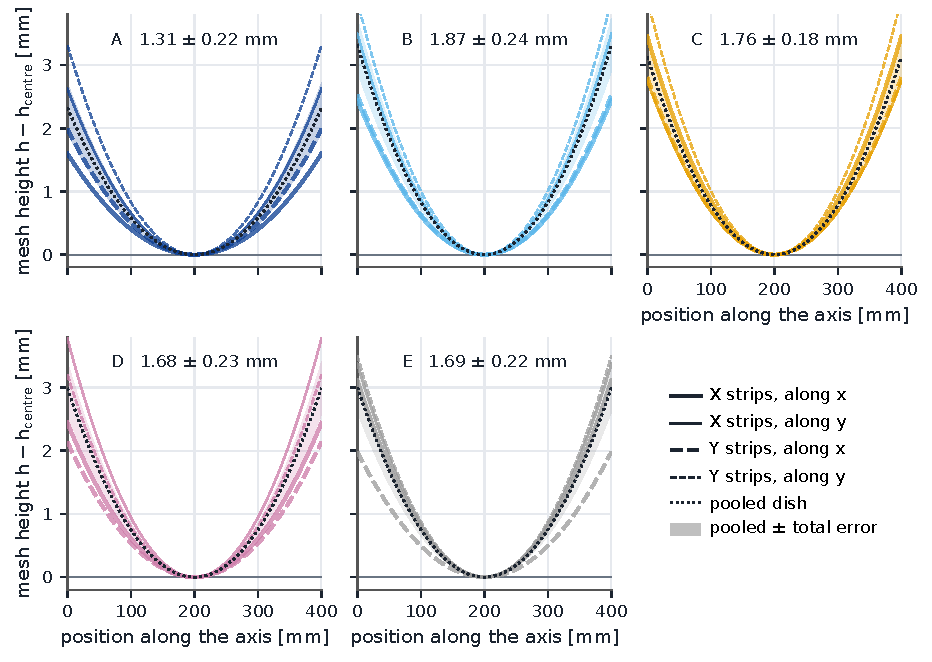
\includegraphics[width=\linewidth]{bow_profiles}
  \caption{Height of the mesh across each chamber from position residuals against the slope of the reference track,
  relative to its centre, one panel per chamber: the fitted quadratic surface, evaluated along $x$ (thick) and $y$
  (thin) through the centre, for the X strips (solid) and the Y strips (dashed), with the rigid tilt removed. Dotted:
  the pooled dish; band: its combined error (bootstrap and the scatter of the four terms). The data behind the
  chamber~A panel are in \crefp{fig:bow}{a, b}.}
  \label{fig:bowprof}
\end{figure}
